\chapter{Introduction}

Nuclear structure has been studied since the late 19th century, but a complete
understanding of the proton's spin has eluded scientists.  Early models of the
proton structure such as the three valence quark model could accurately predict
the charge and spin of the proton. When the spin contribution of the valence
quarks was measured in 1988~\cite{Ashman1988}, their contribution was found to
be much less than the total spin of $1/2$. This event is known as the `proton
spin crisis' (Figure~\ref{fig:spin_crisis_cartoon}).

Although recent papers \cite{Povh2016} have suggested that this `spin crisis'
(Figure~\ref{fig:spin_crisis_cartoon}) is simply due to mis-attribution of
spin, most literature to date has focused on understanding how to model the
proton with parton distribution functions, and the vast scientific consensus is
that the EMC results published detailing the spin crisis in 1988 are valid.

Following the spin crisis, a major challenge in particle physics theory was to
create a framework which could explain both the `valence-quark' behavior of
protons at some scattering energies, as well as predict the break down of that
model and properly account for the proton's spin. Global
analyses~\cite{DeFlorian2009} were undertaken to model the proton with
probabilistic structure functions, incorporating scale-dependent structure.
These global analyses require experimental data as a constraint for the
structure function parameterization. One method of providing constraints is
through the measurement of particle production asymmetries~\cite{Kang2011}.
\clearpage

Structure functions can be used to calculate parton distribution functions,
which describe the momentum fraction carried by partons in the proton. Parton
distribution functions may describe either polarized or unpolarized partons. In
global analyses, the parton distribution functions for quark polarization are
calculated from the structure functions, and experimental data constrains these
functions via the calculation of the asymmetry.

\begin{figure}
  \centering
  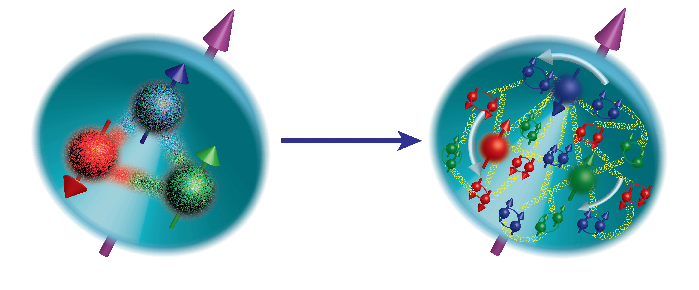
\includegraphics[width=0.8\linewidth]{./figures/figures_introduction_nucleon_picture.png}
  \caption{
    Left: the n{\"a}ive quark model, while predicting the correct spin of the
    proton, does not bear fruit when the quark spin contribution is measured.
    Right: a more realistic cartoon of the proton as a composite of gluons,
    valence quarks and sea-quarks~\cite{Accardi2012}.
  }
  \label{fig:spin_crisis_cartoon}
\end{figure}
 
\section{Scope and Objectives of This Work} 

This thesis seeks to measure the longitudinal asymmetry of the $W\rightarrow\mu$
process in order to provide experimental data to constrain the polarized parton
distribution functions characterizing the anti-quarks in the proton sea.
Additionally, I present an analysis which characterizes the luminosity of the
beams produced at the Relativistic Heavy Ion Collider (RHIC).

I begin by laying out the historical foundations of deep inelastic scattering,
and the larger pursuit to understand the structure of matter in
Chapter~\ref{ch:history}. Then, I describe the theoretical underpinnings of
proton structure, for both unpolarized and polarized parton distribution
functions in Chapter~\ref{ch:modeling_proton_spin}.
Chapter~\ref{ch:experimental_apparatus} contains a description the experimental
apparatus, the Relativistic Heavy Ion Collider (RHIC), and how it is used to
carry out the data acquisition and facilitate this analysis. I will discuss the
Vernier Analysis (Chapter~\ref{ch:vernier_analysis}), and how this relates to
understanding the absolute luminosity delivered by RHIC collisions--an important
parameter needed to normalize any cross section measured experimentally at RHIC.
Chapters \ref{ch:data_analysis}-\ref{ch:spin_analysis} contains a discussion of
the analysis of the data set taken by the Pioneering High Energy Nuclear
Interaction Experiment (PHENIX) at RHIC in 2013.  These chapters motivate the
selection of analysis variables from the data set, the transformations applied
to the data to extract our observable, the longitudinal asymmetry, and the
calculation of the asymmetry itself.  Finally, I will discuss the outlook and
impact of these measurements in Chapter~\ref{ch:conclusion}.
